\chapter{海量数据分析与车辆移动模型建立}

<建模规则概述>

\section{出租车数据介绍}
从“北京智能交通系统关键技术研究与应用示范项目”获取的数据集,该项目以支持智能交通系统工程建设、解决关键技术难题、提升交通科技发展水平和自主创新能力、为实现新北京交通体系和奥运会的顺利召开提供支持与保障为目标。其核心研发内容之一,是实时采集、存储、处理多源异构海量交通数据、形成动态交通信息以及决策支持的分布式处理系统。该项目涉及出租车为12096辆,约占北京市出租车总数的$18\%$,对五环内(含五环)次干路以上路网的覆盖率达到$90\%$以上。通过这些出租车上安装的GPS定位装置,每隔约60s上传一次自己的经纬度位置、速度、方向信息到数据中心。每天产生的数据量约1300万条。
数据记录格式如表\ref{table_dataset}所示。

\begin{table}
\caption{北京市出租车数据格式和字段意义}\label{table_dataset}
\begin{tabular}{l|c}
\hline
列名&	说明\\
\hline
调度中心ID&	4个ASCII字符;\\
\hline
出租公司ID&	标记出租车为何公司所有.\\
\hline
车辆ID&	使用11个ASCII字符;\\
\hline
时间标签&	使用GMT时间格式共14个ASCII字符,格式为(YYYYMMDDHHMMSS);\\
\hline
84坐标系经度&	最长为11个ASCII字符,变长;\\
\hline
84坐标系纬度&	最长为10个ASCII字符,变长;\\
\hline
02坐标系经度&	一般为9个ASCII字符,除以3686400(1024*3600)后变为通用经度坐标;\\
\hline
02坐标系纬度&	一般为9个ASCII字符,除以3686400(1024*3600)后变为通用纬度坐标;\\
\hline
速度&	单位为公里/小时,最长为3个ASCII字符,变长;\\
\hline
方向&	以正北为0度,顺时针方向增大,为0~360角度,最长为3个ASCII字符,变长;\\
\hline
状态&	为1个ASCII字符,数值型字符,包括空载、满载等状态。\\
\hline
事件(event)&	为1个ASCII字符,数值型字符,包括上下车、开锁车门等。\\
\hline
高度&	两个ASCII字符,固定值为50,未使用\\
\hline
\end{tabular}
\end{table}


\section{出租车行为假设}

在日常生活中,我们打车可能需要走到小区或者学校门口,在车站,飞机厂等地也都设有专门的打车区域,基于我们日常生活经验和主观感受,我们提出了以下假设:
%假设1
\begin{assumption}\label{assuption_1}
\textbf{车辆行为与其车辆状态有关。}当一辆出租车处于载客状态时,它的目的地是确定的,其速度会相对增加。相反的,当一辆出租车处于空载状态时,出租车可能会减速甚至停靠在路边来寻找或等待可能的客人。这样,出租车的行为,例如车辆速度和状态持续时间都会随着车辆状态的变化而变化。
\end{assumption}
%假设2
\begin{assumption}\label{assuption_2}
\textbf{车辆的行为与其时间因素有关。}
车辆在不同时间段的上下客的数量可能与时间服从一定的规则。例如,晚上的客人数量会相对于白天的客人有所减少。其与时间的相关性还有可能体现在以下几个方面。
\begin{itemize}
\item 上下客的热点区域可能会随着时间变化而发生变化。
\item 上下课的事件数可能会随着时间的变化而变化。例如凌晨发生载客和下客事件的数量都会相对减少,而到了白天,去往商场,写字楼等热门区域的出租车载客和下客的数量都会明显增多。
\end{itemize}
\end{assumption}
%假设3
\begin{assumption}\label{assuption_3}
\textbf{车辆行为与其地理因素有关。}
当一辆出租车处于载客状态时,出租车的目的地更可能是某些特定区域,例如机场,火车站等。同时,当出租车为空载状态时,出租车更倾向于选择附近的热点区域,在这样的区域内,人们更倾向于打车,例如某些商业街,电影院。车辆行为与地理因素的相关性可能体现在以下方面:
\begin{itemize}
\item 出租车选择目的地点与出租车的当前位置有关。
\item 事件在不同区域发生的概率不同。
\item 不同事件在相同区域发生的概率不同。
\end{itemize}
\end{assumption}

接下来,为了验证我们的假设,我们基于北京市出租车数据对车辆的速度,状态持续时间,

%从数据角度的分析
\section{出租车数据分析}
本节针对本文提出的三个假设,从数据角度予以论证。分别验证出租车行为与车辆状态,时间以及地理因素之间的关系。

%验证1: 出租车状态对速度等的影响
\subsection{出租车行为与出租车状态的关系}

出租车行为可以由一个多元组表示,其中包括多个属性,常见的属性有速度,状态等。本节分析出租车的速度和状态持续时间随车辆状态的变化情况。

如图\ref{figure_speed_distribution}所示的是空载和载客状态下每小时的平均速度情况。由图可以凌晨0点到4点车辆的速度明显低于载客状态下的速度,空载时的速度在$3km/h-20km/s$,而载客时的速度则为$20km/h-40km/h$.在这个时段里车流量上,载客时可以达到较高的车速,而空载时为了降低油耗,空载时司机多选择停靠在路边“等活”。
在早上8点到12点的时段里,空载和载客时的平均速度类似,可能是由于这个时段的车流量的增加,出租车空载和载客时的运行速度都受到限制,而乘客变多,使得出租车空载时有了更多的载客机会,出租车司机会倾向于“扫活”,即沿着马路低速行驶或者快速移动到人群密集的区域。
%图:空载和载客状态下每小时的平均速度
\begin{figure}[ht]
\centering
\begin{tabular}
[c]{c}
\epsfysize=2in\epsfbox{figures/analysis/avgsp_vacant.eps} \\
(a) vacant status \\ 
\epsfysize=2in\epsfbox{figures/analysis/avgsp_occupied.eps} \\
(b) occupied status \\
\end{tabular}
\caption{空载和载客状态下每小时的平均速度}\label{figure_avg_speed}
\end{figure}

本文还选取了几个特定时间段,分析其车辆的空载和载客情况下的速度分布情况。
%图:不同时间段,空载和载客状态下的速度分布情况
\begin{figure}[!h]
\centering
\begin{tabular}
[c]{cc}
\epsfysize=1.5in\epsfbox{figures/analysis/speed6_0.eps} &
\epsfysize=1.5in\epsfbox{figures/analysis/speed6_1.eps} \\ 
\multicolumn{2}{c}{6:00-8:00}\\
\epsfysize=1.5in\epsfbox{figures/analysis/speed11_0.eps} &
\epsfysize=1.5in\epsfbox{figures/analysis/speed11_1.eps}\\
\multicolumn{2}{c}{11:00-13:00}\\
\epsfysize=1.5in\epsfbox{figures/analysis/speed17_0.eps} &
\epsfysize=1.5in\epsfbox{figures/analysis/speed17_1.eps}\\
\multicolumn{2}{c}{17:00-19:00}\\
\epsfysize=1.5in\epsfbox{figures/analysis/speed22_0.eps} &
\epsfysize=1.5in\epsfbox{figures/analysis/speed22_1.eps}\\
\multicolumn{2}{c}{22:00-24:00}\\
(a) vacant status& (b) occupied status\\
\end{tabular}
\caption{不同时间段,空载和载客状态下的速度分布情况}\label{figure_speed_distribution}
\end{figure}

图\ref{figure_speed_distribution}为在对应时间段车辆速度的累积分布情况。其中的一点$(x,y)$表示,速度瞬时速度小于$x~km/h$的速度记录占总数量的$y$.
如图\ref{figure_speed_distribution}所示,载客状态下的速度分布情况与空载情况下的速度分布有较大不同。空载情况下,速度为0的情况达到了$50\%$,而载客情况下速度为0的情况占$25\%$.两者的分布曲线也有较大不同。


%图:状态持续时长分布
从经验来看,出租车司机为了提高收入应该尽可能的降低空载率,因此我们探究了载客持续时长和空载持续时长的情况。图\ref{figure_duration_for_each_status}为状态持续时长的分布情况。可以看出空车时的持续时长偏短,$80\%$的概率,持续时长小于1000秒,而$80\%$的载客时的持续时长小于等于1500秒。
\begin{figure}[ht]
\centering
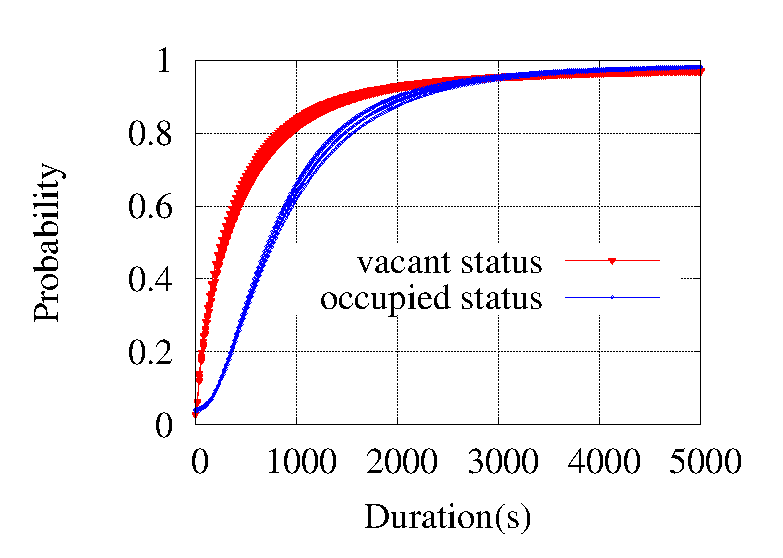
\includegraphics[width=0.5\textwidth]{figures/assumption/durationdis.eps}\\
\caption{状态持续时长分布}\label{figure_duration_for_each_status}
\end{figure}


\subsection{随时间变化的事件分布}
本节我们分析了每小时有多少载客和下客事件发生。每小时的事件数量变化如图\ref{figure_event_varied_w_t}所示,统计结果如表\ref{table_event_distribution_with_time}所示,可以看出一周内载客和下客总量分别为$2,679,385$和$2,707,290$, 两者相差不多。且其中的波峰和波谷的时间段也类似,波峰为11月4日的晚上7点到8点,波谷为11月3日的凌晨4点和5点。出现这样的结果与我们的日常生活经验吻合,因为载客和下客事件具有较强相关性的,两者应该保持动态平衡。同时,图\ref{figure_event_varied_w_t}表明波峰和波谷出现的时间段类似,客流量增加和减少表现出较强的规律性。

\begin{figure}[!h]
\centering
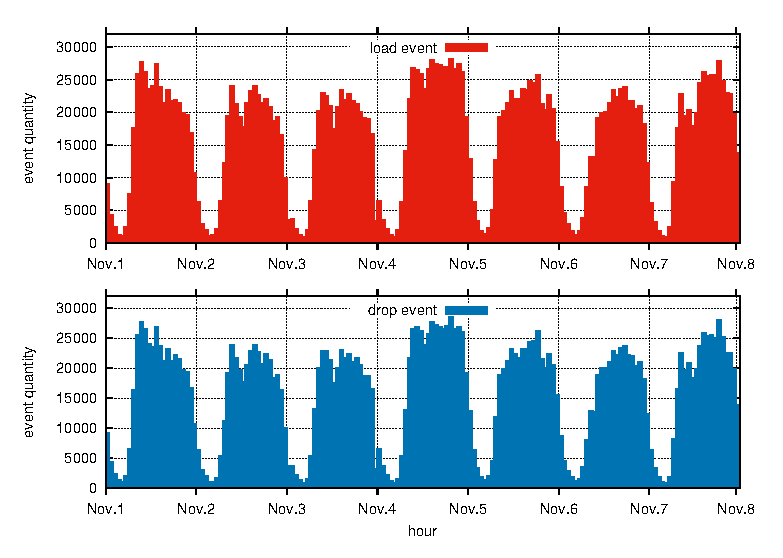
\includegraphics[width=0.65\textwidth]{figures/analysis/event_w_time.eps}\\
\caption{Taxi event varied with time.}\label{figure_event_varied_w_t}
\end{figure}



\begin{table}[!h]
\caption{随时间变化的事件数}\label{table_event_distribution_with_time}
\centering
\begin{tabular}{l|c|c}
 \hline
 名称 & 下客事件数 & 上客事件数 \\
  \hline
  一周总数& 2,679,385&2,707,290\\
  一小时内最大值&28,583 &28,130\\
  一小时内最小值&861&918\\
  波峰时段&11月4日, 19:00-20:00&11月4日, 19:00-20:00\\
  波谷时段&11月3日, 4:00-5:00&11月3日, 4:00-5:00\\
  \hline
  \end{tabular}
\end{table}







\begin{figure}[ht]
\centering
\begin{tabular}
[c]{cc}
\epsfysize=2in\epsfbox{figures/analysis/hotspots/hotspot_drop_04.eps} &
\epsfysize=2in\epsfbox{figures/analysis/hotspots/hotspot_drop_19.eps} \\
(a) drop events at 4:00-5:00 & (b) drop events at 19:00-20:00\\
\epsfysize=2in\epsfbox{figures/analysis/hotspots/hotspot_load_04.eps} &
\epsfysize=2in\epsfbox{figures/analysis/hotspots/hotspot_load_19.eps} \\
(c) load events at 4:00-5:00 & (d) load events at 19:00-20:00\\
\end{tabular}
\caption{一小时内,出租车上下客事件的发生密度}\label{figure_taxi_density_for_one_hour}
\end{figure}




\subsection{出租车行为与地理因素之间的关系}

本节主要验证假设出租车行为与地理因素具有显著关系,出租车的载客和下客事件的分布具有地理偏好。
图\ref{figure_taxi_density_for_one_hour}
\begin{figure}[!h]
\centering
\begin{tabular}
[c]{cccc}
\epsfysize=1in\epsfbox{figures/analysis/hotspots/1hotspot_20_drop_19.eps} &
\epsfysize=1in\epsfbox{figures/analysis/hotspots/3hotspot_20_drop_19.eps} &
\epsfysize=1in\epsfbox{figures/analysis/hotspots/5hotspot_20_drop_19.eps} &
\epsfysize=1in\epsfbox{figures/analysis/hotspots/6hotspot_20_drop_19.eps} \\
(a) 11月1日,周二 &(b) 11月3日, 周四 &(c) 11月5日, 周六 &(d) 11月6日,周日 \\
\multicolumn{4}{c}{下客事件热点区域}\\
\epsfysize=1in\epsfbox{figures/analysis/hotspots/1hotspot_20_load_19.eps} & 
\epsfysize=1in\epsfbox{figures/analysis/hotspots/3hotspot_20_load_19.eps} &
\epsfysize=1in\epsfbox{figures/analysis/hotspots/5hotspot_20_load_19.eps} &
\epsfysize=1in\epsfbox{figures/analysis/hotspots/6hotspot_20_load_19.eps} \\
(e) 11月1日,周二 &(f) 11月3日, 周四 &(g) 11月5日, 周六 &(h) 11月6日,周日 \\
\multicolumn{4}{c}{载客事件热点区域}\\
\end{tabular}
\caption{出租车一小时内载客和下客事件的数量的区域分布}\label{figure_taxi_density_for_one_hour}
\end{figure}

图~\ref{figure_taxi_desity_for_one_hour} 在同一时间段内(19:00到20:00)表明载客/下客事件的热点区域(一小时内事件发生超过20次的区域)。我们选择了两个工作日和一个周末进行比较。通过比较载客和空载的热点,我们发现载客事件分布相对于空载事件比较平均。

对于每种事件分布,热点区域的出现具有会重复出现,热点见图~\ref{figure_taxi_desity_for_one_hour}中红圈表明的地方。
虽然工作日和周末的事件数有所变化,但是热点区域出现的地点还是类似的。
这种现象的出现可能是由于载客事件主要分布在居民的家中,而下客地点更趋向于聚集在工作地点,地铁站或者风景区。
 
 总的来说,在每个网格内的载客和下客数量变现出地理特征:
 \begin{itemize}
  \item 事件分布不均匀,载客和下客事件的分布有所不同。
  \item 对于某种状态,热点区域出现具有可重现性,在某些标志性区域(北京西站,国贸等地)重复出现。
\end{itemize}

综上所述,可以证明假设三具有一定的合理性,即出租车行为与地理因素有关。


\section{建立模型}

移动模型定义了节点的运动模式$Paths:<p_1,p_2…,p_n>$,$p_i$的确定可以简化为两步,即,目的地点选择和从源地点到目的地点的移动模式。
目的地点选择:节点的目的选择也与节点的当前状态有关。若节点处于载客状态。若当前状态为载客状态:针对载客事件将区域划分为不同的子区域,同理由下客事件分布将区域划分为不同的子区域。计算由载客子区域到下客子区域的转移概率矩阵和距离范围。然后由节点当前位置,决定下客位置。同理,节点处于下客状态时,由当前位置,和区域转移矩阵也可以计算得到载客的目的节点。

\subsection{地图抽取}

\begin{figure}[!h]
\centering
\fbox{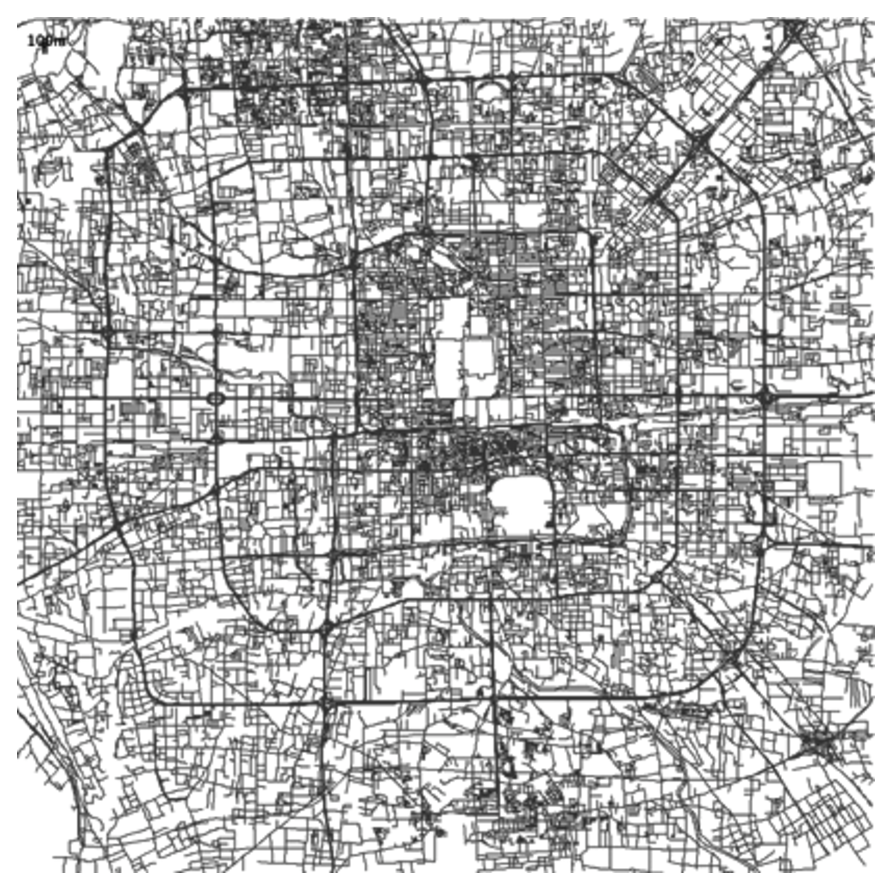
\includegraphics[width=0.4\textwidth]{figures/map.eps}}\\
\caption{抽取地图}\label{figure_map}
\end{figure}


\subsection{区域定义与识别}
lalal


\subsection{区域转移概率}
区域转移概率


\subsection{速度建模}
\begin{figure}[!h]
\centering
\begin{tabular}
[c]{cc}
\multicolumn{2}{c}{6:00-8:00}\\
\epsfysize=1.5in\epsfbox{figures/evalue/fitspeed6_0.eps} &
\epsfysize=1.5in\epsfbox{figures/evalue/fitspeed6_1.eps} \\
\multicolumn{2}{c}{11:00-13:00}\\
\epsfysize=1.5in\epsfbox{figures/evalue/fitspeed11_0.eps} &
\epsfysize=1.5in\epsfbox{figures/evalue/fitspeed11_1.eps} \\
\multicolumn{2}{c}{17:00-19:00}\\
\epsfysize=1.5in\epsfbox{figures/evalue/fitspeed17_0.eps} &
\epsfysize=1.5in\epsfbox{figures/evalue/fitspeed17_1.eps} \\
\multicolumn{2}{c}{22:00-24:00}\\
\epsfysize=1.5in\epsfbox{figures/evalue/fitspeed22_0.eps} &
\epsfysize=1.5in\epsfbox{figures/evalue/fitspeed22_1.eps} \\
(a) vacant status & (b) occupied status \\
\end{tabular}
\caption{速度分布的拟合结果}\label{figure_fitspeed_varied_with_time}
\end{figure}



为了获取各个状态的速度分布,我们对瞬时速度的累积分布进行拟合,以获取瞬时速度的累积分布函数,然后衍生出其速度分布函数。
由图\ref{figure_fitspeed_varied_with_time}可知,除了载客状态时从22:00-24:00的累积瞬时速度分布外,瞬时速度的累积分布表现出指数分布的规律,拟合函数记为$f_1(x)$。载客状态时从22:00-24:00的累积瞬时速度分布表现出线性分布的特性,其拟合函数记为$f_2(x)$, 如公式\ref{formular_ccdf_speed}。由分析过程可知,某些天,例如周末的某些时段会影响车辆的行为,我们仅分析最常见的情况,因此去掉了明显不一样的情况,例如周六和周天早上6点到8点时的载客状态的累积速度分布。

\begin{equation}\label{formular_ccdf_speed}
\left\{
\begin{array}{ll}
f_1(x) = 1-1/exp(-ax^b-c)\\
f_2(x) = ax+b
\end{array}
\right.
\end{equation}

\begin{table}[ht]
\caption{拟合参数以及拟合曲线的残差平方和}\label{table_rms}
\centering
\begin{tabular}{c|c|c}
  \hline
  时间段 & 空车状态 & 载客状态 \\
  \hline
6:00-8:00   &0.0129207 & 0.019818 \\
11:00-13:00 &0.00866176 & 0.0204889 \\
17:00-19:00 &0.0176578 & 0.0105868 \\
22:00-24:00 &0.0154822 & 0.0240426 \\
  \hline
\end{tabular}
\end{table}

拟合结果以及相关的残差平方和(root mean square, rms)如表\ref{table_rms}所示,越小的残差平方和代表越小的误差。由表\ref{table_rms}可知,所有的残差平方和均小于$0.025$,表现出较好的拟合相似性。


\section{本章小结}
tete

